\section{Informationstechnischer Aufbau}
\label{sec:Informationstechnischer Aufbau}

\begin{figure}[htb]
\centering		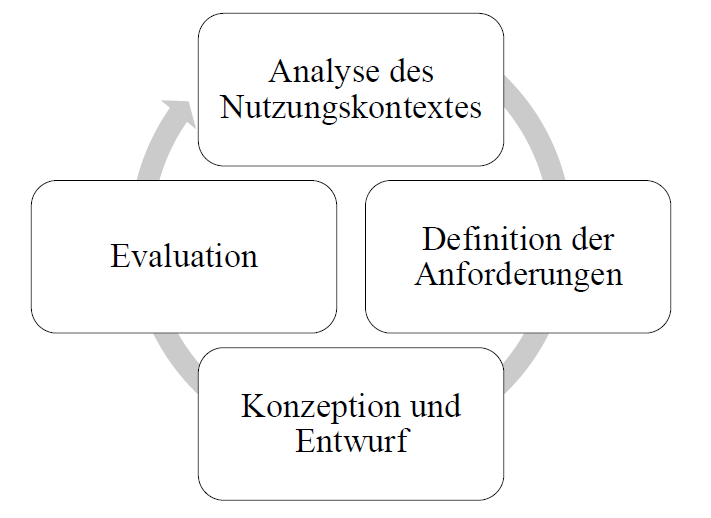
\includegraphics[width=0.50\textwidth]{Pictures/UCD.png}
\caption{Prozesschritte beim \textit{User Centered Design} \citep{Nuerenberg2015}}
\label{fig:}
\end{figure}

In diesem Abschnitt wird der informationstechnischer Aufbau der KA vorgestellt und erläutert. Eine Grundlage für die Software-Entwicklung für die KA war das Vorgehen und Erfahrungen aus dem Aufbau der Klimakammer und dessen SPS-Entwicklung. Das Grundgerüst für die SPS bildet die Ablaufstruktur aus dem Klimakammer-Projekt und sind nachzulesen in \textsc{\citeauthor{Nuerenberg2015}}. Das Konzept wurde an die Anforderung der KA angepasst sowie in einigen Teilen weiterentwickelt und um neue Programme und Ablaufstrukturen ergänzt. Zunächst wird das Grundkonzept sowie das Vorgehen erläutert, um später auf die Konzepte und Teilprogramme näher einzugehen. 

\subsection{User Centered Design(UCD)}
\label{subsec: UCD}

Für das Vorgehen der Software-Entwicklung für die KA ist der Ansatz des \textit{User Centered Design} (UCD). Dieser Ansatz dient zur Gestaltung von interaktiven System. Im Mittelpunkt stehen hierbei die Bedürfnisse, Fähigkeiten und Erfahrungen vom Endanwender stehen. Es wird sowohl für die Produktentwicklung als auch in der Softwareentwicklung eingesetzt. Sie beruht auf der alten Norm  EN ISO 13407 \footnote{EN ISO 13407: Benutzer-orientierte Gestaltung interaktiver Systeme} und ging in der neuen Norm EN ISO 9241-210 \footnote{EN ISO 9241-210: Prozess zur Gestaltung gebrauchstauglicher interaktiver Systeme}  auf. \citep{Normung2010}

Das Konzept besteht aus vier Prozessschritten. Zunächst wird in der \textit{Analyse des Nutzungskontextes} die Benutzergruppe, ihr fachlicher Hintergrund und ihre Arbeitsaufgaben definiert. Bei der Benutzung der KA handelt es sich um Entwickler oder um eingewiesenes Personal. Beide verfügen über gutes bis sehr gutes technisches und thermodynamisches Verständnis. Sie kennen die Funktionen der einzelnen Bauteile und das Verhalten des Prüfstandes. Technisches Fachtermini sowie englische Begriffe werden vorausgesetzt.  Des Weiteren verfügt er über Erfahrungen im Umgang mit PC-Software.

Nach der Definition und Analyse des Nutzungskontextes folgt die nächste Phase der \textit{Definition der Anforderungen}. Die Anforderung der Software werden festgelegt und danach in zwei Untergruppen unterteilt. Die eine Untergruppe beinhaltet alle Aufgaben die vom Benutzer ausgeführt werden. Die andere Untergruppe definiert alle Aufgabenfelder die von der Technik ausgegührt werden sollen. 
Vom Benutzer werden die folgenden Arbeitsfelder durchgeführt:
\begin{itemize}
\item	Messen
\item	Steuern und Regeln
\item	Beobachten und Analysieren
\item	Optimieren.
\end{itemize}

Um diese Arbeitsfelder durchführen zu können, werden die \textit{Basisanforderungen} an die Software definiert. Diese umfassen die Sicherheit für Mensch und Maschine, ein effizientes und konfortables Arbeiten. Zuletzt soll die Software flexible und erweiterbar sein. 

Nach der Erfassung der Anforderungen geht die Software-Entwicklung zur nächsten Phase über, die \textit{Konzeption und Entwurf}. In der Arbeit von \textsc{\citeauthor{Neumann2007}} \citep{Neumann2007} werden zu beachtende Gesetze für diese Phase aufgelistet. Diese Gesetze sollen ein späteres effizientes, angenehmes Arbeiten ermöglichen. In \citep{Preim2013} werden 15 Punkte genannt, die es bei der Entwicklung einer ergonomischen Softwareentwicklung zu berücksichtigen gilt.

Die letzte Phase des UCD ist die kontinuierliche \textit{Evaluation} der Software. Der Kreis des UCDs ist nun geschlossen und fängt von Vorne an. Es ist ein kontinuierlicher Prozess für eine bessere und effizientere Software für die definierten Aufgabenfelder. 

\subsection{Statusmaschine}
\label{subsec:Statusmaschine}

Die Statusmaschine ist das Werkzeug zur Umsetzung der vom UCD definierten Basisanforderungne der KA-Software. Das Werkzeug für eine kontinuierliche und zuverlässige Ausführung der Anforderungen ist eine Speicher-Programmierbare-Steuerung (SPS) am besten geeignet. Die SPS gewährleistet sowohl die kontinierliche Ausführung des Programm-Codes und besitzt eine hohe Kompatibilität mit der eingesetzten Hardware inklusive Regler und Sensoren der KA. 

Die SPS ermöglicht desweiteren das Lesen und das Schreiben jeder Variablen innerhalb eines Zykluses. Ein herkömmliches PC-Programm ist, im Gegensatz zu dem  zyklusgesteuerten SPS-Programmcodes, ereignisgesteuert. Die Dauer für einen Durchlauf des Programmes in einem herkömmlichen PC-Programm variiert je nach Belegung des Arbeitsspeicher und Auslastung des CPUs. Der Ablauf einer zyklusgesteuerten SPS lässt sich unterteilen in folgende Teilschritte:

\begin{enumerate}
\item	Nach Bereitschafts-Kontrolle aller angeschlossenen Baugruppen wird das Prozessabbild aller Eingänge aktualisiert. Der Status aller Eingangs-Busklemmen werden abgefragt
\item 	Die SPS gibt die Kontrolle an den Anwender-Code und durchläuft diesen. Als Ergebnis entsteht ein neues Prozessabbild der Ausgänge. 
\item	Die Kontrolle wird nun wieder an das Betriebssystem der SPS übergeben und diese gibt das Prozessabbild weiter an die Busklemmen. 
\end{enumerate}


\begin{figure}[htb]
\centering		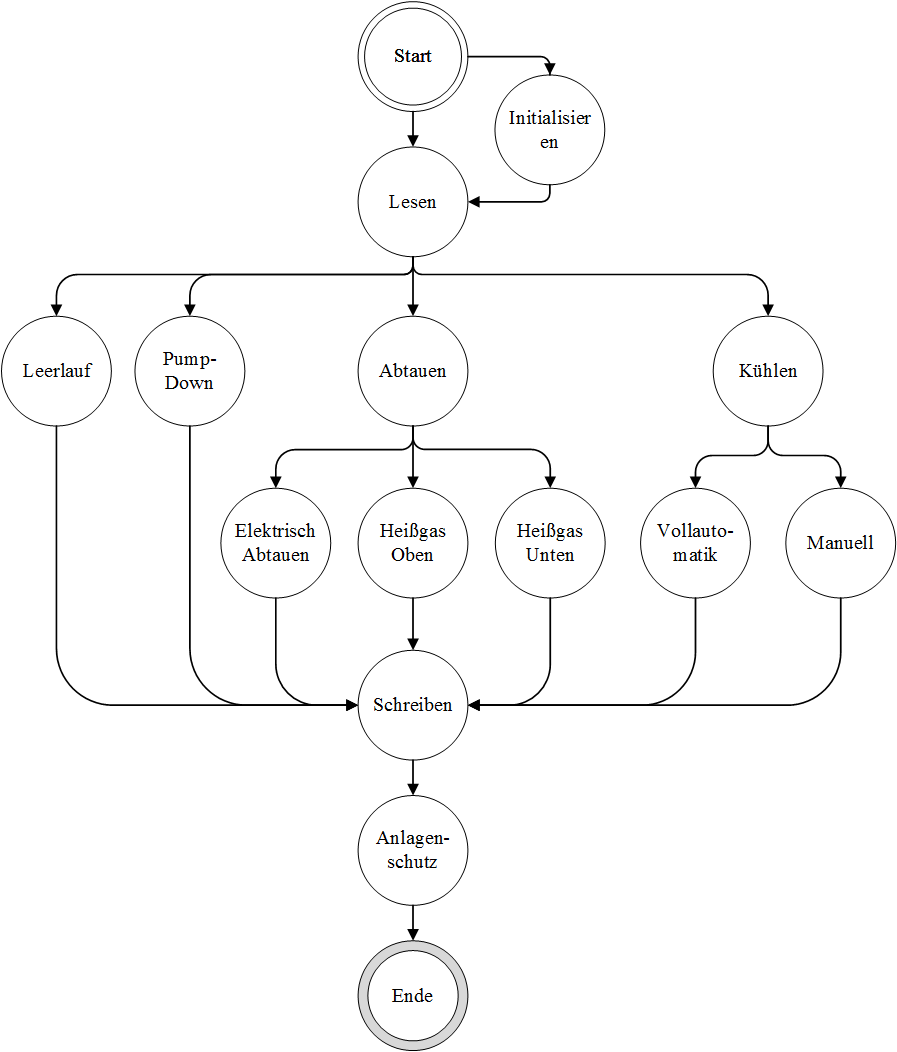
\includegraphics[width=0.85\textwidth]{Pictures/SM.png}
\caption{Statusmaschine}
\label{fig:SM}
\end{figure}


Nachdem alle Teilschritte durchlaufen sind, beginnt der Zykus von Vorne. Die Zeiten für einen Zyklus variierten je nach Anwendung und können vom Benutzer eingestellt werden. Die zyklische Verarbeitung von einem Programmcode kann dazu führen, dass Funktionen Ergebnisse gegenseitig beeinflussen oder den Wert einer Variable öfters überschrieben werden könnte. Deshalb wird das Konzept einer sogenannte Statusmaschine verwendet. Eine Statusmaschine orientiert sich dabei an der grundsätzlichen Ablaufstruktur einer zyklusgesteuerten SPS. Das Verwenden einer Statusmaschine erleichtert eine gegenseitige Beeinflussung der verschieden Zustände der Statusmaschine. 

Die Verwendung eine Statusmaschine verkürzt den zu durchlaufenden Programmcode und erleichert eine Fehlersuche und -analyse. Des Weiteren ist eine Statusmaschine leichter zu designen, nachzuvollziehen und zu diskutieren. Das Abbild \ref{fig:SM} verdeutlicht den Aufbau des Statusmaschine-Konzeptes. 

Die Statusmaschine beginnt ihren Zyklus beim Start. Dort wird über eine Transitionsvariable entschieden, ob die Prozessparameter neu initialisieren werden sollen. Ist dies nicht der Fall so wird sofort in den Status \textit{Lesen} gewechselt. Im weiteren Verlauf entscheiden weitere Transitionsvariablen über den nächsten Zustand der Statusmaschine.  

\subsubsection*{Statusmaschine: Initialisieren}

Während der Initialisierungsvorgangs werden Daten aus den Datenbanken eingelesen und an die Variablen weitergegeben. Das Konzept der Datenbanken beruht hauptsächlich auf dem Programm $DB\_lesen$ von \textsc{\citeauthor{Nuerenberg2015}}\citep{Nuerenberg2015}. 
Die Verbindung zu einer Tabelle aus der Datenbank wird mittels des Funktionsblockes \textit{FB$\_$DBRecord-ArraySelect} hergestellt. Aus der Tabelle werden dann eine bestimmte Menge an Datensätzen liest. 
Die Verbindungsinformationen zur Datenbank und Tabelle werden über das Beckhoff-Konfigurationstool \textit{Database Server Konfigurator} hergestellt und verwaltet. 
Rückgabewert des Funktionsbausteins $FB\_DBRecord-ArraySelect$ ist ein Array der Struktur der Tabelle. Bei keinem Fehler ist die Tabelle mit Werten von der Datenbank gefüllt und die Größe des Array größer als Null. Kam es zu einem Verbindungsfehler, konnten die Daten nicht eingelesen werden und die Arraygröße ist gleich Null. Dann wird die Fehler-Boolvariable $bDBFehler$ auf TRUE gesetzt und die Statusmaschine verharrt im Status \textit{Initialisieren}. 

Das gefüllte Array mit den Tabellenwerten wird im folgenden Schritt an die lokale Struktur übergeben. \textsc{\citeauthor{Nuerenberg2015}} verwendet hierzu eine Kombination aus einer FOR-Schleife mit einer IF-Abfrage. Mit der FOR-Schleife wird die ID-Nummer hochgezählt und falls der Variablenname mit dem lokalen Namen übereinstimmt in deren Struktur übergeben.  
\textsc{\citeauthor{Nuerenberg2015}} schreibt in seiner Arbeit von Problemen mit der Verbindung zur Datenbank in dem ersten Zyklus und setzt daher einen \textit{Timer} ein. Der \textit{Timer} startet den Lese-Prozess nach 3 Sekunden nach dem Start der Statusmaschine und fängt an die Datensätze zu lesen. In dem jetztigen Programmablauf wurde das Timeout für den Funktionsbaustein auf 150 ms gestellt und auf den \textit{Timer} verzichtet. Das führt dazu, dass das System der Kommunikation zwischen SPS und Datenbank mehr Zeit gibt, bevor der Prozess abgebrochen wird und die Fehlervariable auf TRUE gesetzt wird. Dies hat den gleichen Effekt wie der Einsatz eines Timers. Die Datenbanken werden jedoch im ersten Zyklus ausgelesen. 

Stoffwerte, die mittels Datenbankübertragung, an die SPS geliefert werden, sind lokal als \textit{Persistente Variablen} gespeichert. Neukompilieren, Neustarten der SPS oder Progammänderungen haben keinen Einfluss auf die Varialenwert. Die SPS speichert die Variablen lokal auf ihrem Speicherplatz. Dadurch werden die Daten für die Stoffwerte nur dann gelesen, wenn der Benutzer dies mittels der Boolvariable \textit{bLeseStoffwerte} entscheidet. Im Gegensatz zu den anderen Datenbanken, beispielsweise mit Reglereinstellungen, verändern die Stoffwerte sich nicht. Deshalb müssen diese nicht jedes mal beim Starten der SPS gelesen werden. Wird die Stoffwerte Tabellen in der Datenbank angepasst bzw. das Abfrageraster der Werte verkleinert, so muss man die lokalen Strukturen und Iterationsverfahren daran anpassen. 

Desweitern wird während Initialisierung der Status des Wägesystems kontolliert. Sind die Waagen korrekt mit 2 kg vorbelastet, jede Feder gewichtskalibiert und der alle Offsets ermittelt, wird die Boolvariable  \textit{bWaagenBereit} auf TRUE gesetzt. Diese Abfrage gilt nur zur Kontrolle. Das System startet auch ohne die vorher aufgelisteten Schritte, die im Status \textit{Leerlauf} durchgeführt werden. 


Nach erfolgreichem Abschließen geht die Statusmaschine in den nächsten Status: \textit{Lesen}.

\subsubsection*{Statusmaschine: Lesen}

Im Status \textit{Lesen} werden folgende Schritte durchgeführt: 

\begin{itemize}
\item	Temperatur-Eingänge werden ausgelesen
\item	Waagen-Eingänge werden aus Datenpuffer gelesen, vgl. Abschnitt \ref{subsubsec:Modus}
\item	Ablaufstruktur für Modbus RTU, vgl. \ref{subsec:Modbus RTU}
\item 	Berechnungsprogramm für Enthalpien der Zustandspunkte(vgl. Abschnitt \ref{subsec}) sowie 2-D Schwerpunkt der Eismasse im Luftkühler
\end{itemize} 

 die Klemmenwerte der Busklemmen gelesen und in native Werte umgerechtet, zB. 4..20 mA oder 0..10V. Die ermöglicht einen komfortableres und effizienteres Arbeiten und Verarbeiten der Signale auf Seiten des Benutzers. Die Umrechnung von Klemmenwerte (\textit{INT$\_$VAR}) in native Werte(\textit{REAL$\_$VAR}) erfolgt über eine einfache Gradengleichung mit den Parameter \textit{PARA$\_$M} als Gradensteigung und \textit{PARA$\_$C} als y-Achsenabschnitt :

\begin{equation}
REAL\_VAR = PARA\_M\cdot INT\_VAR + PARA\_C; 
\label{eq:SPSNativ}
\end{equation}

\textsc{\citeauthor{Nuerenberg15}}  benutzt für die Umrechnung \ref{eq:SPSNativ} die Funktion \textit{FB$\_$SPS$\_$zu$\_$Nativ$\_$lin}. Die Parameter und die Gradengleichung in der Datenbank für die jeweilige Struktur hinterlegt. Für Eingangswerte wurde die  \textit{INPUT$\_$VAR} und für Ausgangswerte \textit{OUTPUT$\_$VAR} eingeführt. Die Umrechnung von nativen Werten in Klemmenwerten erfolgt im Schritt \textit{Schreiben}.

\subsubsection*{Statusmaschine: Leerlauf}

Ist keine Transitionsvariable beim Start der SPS ausgewählt, so geht die SPS automatisch nach dem Status \textit{Lesen} in den Status \textit{Leerlauf} über. In diesem Status sind alle Komponenten der KA spannungsfrei geschaltet und alle Regler nicht aktiv. In diesem Status wird zu Beginn jeder Messung das Wägesystem kalibriert werden und dann kann zur Messung übergegangen werden. Der genaue Kalibrierungsablauf ist in Abschnitt  \ref{sec:Kalibrierung Wägesystem} beschrieben. 

Befindet die Anlage sich im Kühl- bzw. Abtau-Modus und dieser wird manuell oder automatisch durch den Anlagenschutz abgebrochen bzw. beendet, so geht die Anlage in den sicheren Betriebsmodus \textit{Leerlauf}.  

Nach dem \textit{Leerlauf} geht die SPS in den Status \textit{Anlagenschutz} über.  

\subsubsection*{Statusmaschine: Pumpdown}

Der Status \textit{Pumpdown} bewirkt ein Absaugen des Kältemittels aus dem Verdampfer, um mögliche Kältemittelverlagerungen während einer Stillstandsphase vorzubeugen (vgl. \citep{Siemens2007a}).  Das Kältemittel wird durch den Kompressor angesaugt, durch den Verflüssiger kondensiert und dann unter hohem Durck in den Sammler gedrückt. Damit kein weiteres Kältemittel aus dem Sammler in den Verdampfer nachströmt, bekommt das Expansionsventil per Modbus den Befehlt zum Schließen. Das geschlossene Expansionsventil verhindert weiteres Eindringen des Kältemittels in den Verdampfer. Der Druck sinkt auf der Niedrigdruckseite und steigt auf der Hochdruckseite. 

Der Pumpdown führt zu einem starken Temperaturabfall in dem Verdampfer und den Rohrleitungen, sodass Temperaturen bis zu -20 $°C$ erreicht werden. Um zu starke Unterkühlungen zu verhindern wird der Kompressor beim Pumpdown mit der niedrigsten Drehzahl bei 4 mA betrieben. Fällt der Niedrigdruck vor dem Kompressor unter 1,5  bar, so ist der Pumpdown abgeschlossen.

Für die Schaltung der Schaltschütze zur Spannungsfreigabe sowie Schaltung der Magnetventile wurde der Funktionsbaustein \textit{FB$\_$Schuetzstellung} programmiert. Der Funktionsbaustein hat als Input-Variable \textit{myStatus}, die vom \textit{TYPE}  \textit{Status$\_$Schuetzstellung} ist. Der \textit{TYPE}  \textit{Status$\_$Schuetzstellung} beinhaltet sechs verschiedene Schaltungssituationen:

\begin{itemize}
\item	\textit{KuehlenOben}
\item	\textit{AnlagenPumpDown}
\item	\textit{AnlagenPumpDown$\_$rev}
\item	\textit{AbtauenOben}
\item	\textit{AbtauenUnten}
\item	\textit{AbtauenElektrisch}
\end{itemize}

Dieser Funktionsbaustein ist als Globale Variable deklariert und kann so aus jedem Programm aufgerufen werden. Dies ermöglicht dem Benutzer die Schaltung der elektrischen Bauteile ohne die genauen Schaltpläne nachvollzogen zu haben und vermeidet Fehler bei der Programmierung. 

Um einen Pumpdown durchführen zu können werden die Transitionsvariablen \textit{bPumpDown} und \textit{bPumpdown$\_$rev}  auf TRUE gesetzt. Die Statusmaschine durchläuft nun bei jedem Zyklus den Pumpdown-Status. Unterschreitet der Saugdruck die 1,5 bar ist der Pumpdown erfolgreich abgeschlossen. Die Transitionsvariablen \textit{bPumpdown} und \textit{bPumpdown$\_$rev} werden wieder auf FALSE gestellt und die Variable \textit{bPumpDownAbgeschlossen} bzw. \textit{bPumpDown$\_$revAbgeschlossen} auf TRUE. Der Funktionsbaustein \textit{Status$\_$Schuetzstellung} schaltet automatisch alle Komponenten spannungsfrei. Die Anlage wird neuinistialisiert, um die Sollwerte für den Kühlmodus wieder zu laden und an die lokalen Strukturen weiterzugeben. 

Der Pumpdown kann sowohl bei normaler Strömungsrichtung durchgeführt werden, um den Verdampfer in der KK zu entleeren. Es ist aber auch ein umgekehrter Pumpdown(\textit{AnlagenPumpDown$\_$rev}) implementiert. Dieser erlaubt es das Kältemittel der Hochdruckseite abzusaugen und in den Sammler über den Verdampfer in der KK zu pumpen. Der normale Pumpdown wird nach einer Vereisungsphase vor dem Abtauen, aber auch vor dem Ausschalten der KA automatisch ausgeführt bzw. manuell betätigt. 

Der umgekehrte Pumpdown kann in manchen Situation aktiviert werden, führt mit unter aber zu unerwünschten Betriebsbedingungen, siehe hierzu Abschnitt \ref{cha:Inbetriebnahme}. 

Der nächste Status ist \textit{Anlagenschutz}.

\subsubsection*{Statusmaschine: Abtauen}

Der Status \textit{Abtauen} ruft zwei Programme auf:\textit{ Regelung()} und \textit{Abtauung()}. 

Das Abtauprogramm orientiert sich  an der Empfehlung für den Abtauprozesses des Forschungsrates für Kältetechnik für die verschiedenen Abtaumethoden. Es hat die CASE-Struktur, um einen effizienteren Programmcode, aber auch die Verständlichkeit und Fehlersuche zu optimieren. Die CASE-Struktur ist in Teilschritte unterteilt, die ihren Programmcode ausführen und dann in den nächsten Teilschritt, soweit die Bedingungen dafür erfüllt sind,  übergehen. Je nach Abtaumethode wird die CASE-Struktur anders durchlaufen. Gleich  bei allen Vorgängen ist, dass zunächst ein PumpDown durchgeführt wird und dann die Abtaumethode für das Abtauen geregelt wird. Bei der elektrischen Abtauung ist das Kriterium für ein erfolgreiches Abtauen die Überschreitung von 10 °C vom Temperaturfühler im vereisten Verdampfer. 

Bei der Heißgas-Abtauung ist die vorgegebene \textit{Abtaudauer} entscheidend. Sie wird von dem Benutzer festgelegt und solange wird der Verdampfer mit Heißgas durchströmt. Ist die Zeit abgelaufen wird der Kompressor ausgeschaltet und in den nächsten Teilschritt übergegangen. 

Wurde der Abtauvorgang erfolgreich abgeschlossen oder durch den Benutzer abgebrochenn, werden alle Bool-Variablen, Timer und Komponenten zurückgesetzt bzw. spannungsfrei geschaltet. Die gesamte Abtaudauer wird an die Variable \textit{LetzteAbtaudauer} übergeben. 


Der nächste Status ist der \textit{Anlagenschutz}, es sei denn der der Abtauvorgang wird durch die Transitionsvariable \textit{bAbtauenAbbrechen} abgebrochen. In diesem Falle werden alle Komponenten spannungsfrei geschaltet. Alle Abtau-Transitionsvariablen werden auf FALSE gestellt. Der nächste Status ist der \textit{Leerlauf}. 

\subsubsection*{Statusmaschine: Kühlen}

Der Status \textit{Kühlen} wird eingeschaltet sobald die Transitionsvariable \textit{bKuehlen} auf TRUE gesetzt worden ist. Im Kühlmodus findet die Vereisung des Verdampfers statt. Er besitzt 2 Modi. Der erste automatisch aktivierte Modus ist der \textit{Vollautomatikmodus}; der zweite Modus ist der \textit{Manuellen Modus}. 
Im \textit{Vollautomatikmodus} sind alle Regler \textit{aktiv} sowie der Kompressor und die Ventilatoren von Verflüssiger und Verdampfer sind an. 
Im \textit{Manuellen Modus} besteht die Möglichkeit Regler einzelnd zu testen oder zu parametrieren. Alle Regler und Komponenten der KA sind aus. Der Benutzer kann diese manuell einschaltet und regeln. Außerdem hat er die Möglichkeit den Anlagenschutz zu umgehen, indem er die Transitionsvariable \textit{bAnlagenschutzModus} auf FALSE setzt. Initialisiert wird die Boolvariable jedoch mit TRUE. Der Anlagenschutz greift in diesem Falle nicht. Deshalb sollte diese Option mit äußerster Vorsicht bedient werden. Der nächste Status ist in diesem Falle \textit{Schreiben}. 

Im \textit{Kuehlen}-Status wird nun auch die Transitionsvariable \textit{bVollautomatikModus} auf TRUE gesetzt. In beiden Modi laufen zwei Hauptprogramme:

\begin{itemize}
\item	Regelung()
\item 	Vereisung()
\end{itemize}

Das \textit{Regelung()}-Programm ist wie in den anderen Zustände verantwortlich für die Regelung der PID-Regler, vgl \ref{subsec:Programme}. 
Das Programm \textit{Vereisung()} stellt den Status des Funktionsbaustein \textit{FB$\_$Schuetzstellung} auf \textit{Kuehlen} und startet den \textit{TimerVereisung} mit der \textit{Vereisungszeit}, die vom Benutzer eingestellt wird. Nach Ablauf dieser \textit{Vereisungszeit} wird der Vereisungsvorgang nicht beendet, sondern lediglich eine Meldung als STRING in die Variable \textit{Mitteilung} geschrieben. 

\subsubsection*{Statusmaschine: Anlagenschutz}
Für den Betrieb einer Maschine, in diesem Fall einer KA, ist ein Anlagenschutz unabdingbar. Er ist essentiell für die Sicherheit von Mensch und Maschine. Nach einer Risikomanagementanalyse wurden verschiedene Szenarien entworfen und über Faktoren die \textit{Wahrscheinlichkeit} und \textit{Schaden} das resultierende Risiko berechnet. 
Bei einem unvertretbar hohen Risiko müssen Maßnahmen zur Reduzierung getroffen werden. Diese Maßnahmen können sowohl hardware-technische und software-technischer Natur sein. Hier werden die Schutzfunktionen auf der Software-Seite aufgezeigt:

\begin{itemize}
\item Unter- und Überdruckschutz
	\begin{itemize}
		\item Die KA kann nur in einem Druckbereich von 1 bis 15 		bar betrieben werden. Bei Unter- bzw. Überschreitung 				wird der Kompressor ausgeschaltet. 
	\end{itemize}
\item Überhitzungsschutz für den Kompressor
	\begin{itemize}
		\item Die Ausgangstemperatur beim Kompressor darf im 						Betrieb nicht die 90 °C überschreiten. Ist dies 					der Fall, so wird die Anlage gestoppt und in den 				\textit{Leerlauf} versetzt. 
	\end{itemize}
\item Überhitzungsschutz für den Verdampfer
	\begin{itemize}
		\item Wird die Temperatur von 80 °C  im Verdampfer 						überschritten, kann es zu Rohrrissen im 							Wärmeübertrager kommen und Kältemittel austreten. 					Bei Überschreitung wird die Anlage in den 							\textit{Leerlauf} versetzt und alle Komponenten 					ausgeschaltet. 
	\end{itemize}
\item Sensorausfall
	\begin{itemize}
		\item Fällt ein Drucksensor aus, so ist der 						Anlagenschutz nicht mehr garantiert, deshalb wird die 				Anlage gestoppt und in den \textit{Leerlauf} versetzt. 				Ein Betrieb der Anlage ist nur möglich, wenn alle 					Sensoren einwandfrei funktionieren.  
	\end{itemize}
\item Sensorschutz Waagen
	\begin{itemize}
		\item Die Waagen sind bis zu einer Belastung von 10 kg 				ausgelegt. Eine Überlastung könnte zu einer Zerstörung 				des Dehnungsstreifen führen. Deshalb wird im Falle einer 		Vereisung, eine elektrische Abtauung eingeleitet, um die 		Waagen zu entlasten. 
	\end{itemize}
\end{itemize} 

Nach dem Anlagenschutz folgt der Status \textit{Schreiben}.


\subsubsection*{Statusmaschine: Schreiben}

Der Status \textit{Schreiben} dient zur Übertragung des Prozessbildes  nach dem Durchlaufen des Zykluses an die Ausgangsklemmen. Hierfür werden die nativen Werte wieder zurück in Integer-Klemmenwerte umgerechnet.

Die Gleichung \ref{eq:NativSPS} zeigt an dem Beispiel für die Umrechnung des Sollwertes für den Kompressor $Soll\_KP$

\begin{equation}
Soll\_KP.INT\_VAR\_Output = \frac{Soll\_KP.REAL\_VAR - Soll\_KP.PARA\_C}{Soll\_KP.PARA\_M}.
\label{eq:NativSPS} 
\end{equation}

Für diese Berechnungsformel setzt \textsc{\citeauthor{Nuerenberg2015}} die rekursive Funktion $FB\_Nativ\_zu\_SPS\_lin$ ein. Die Umrechnung der Sollwerte erfolgt in den Programmen \textit{SchreibeSollwerte()}. Der nächste Status ist \textit{Lesen} bzw. \textit{Initialisieren}.

\subsection{TwinCAT 3}
\label{subsec:TwinCat}

\begin{figure}[htb]
\centering		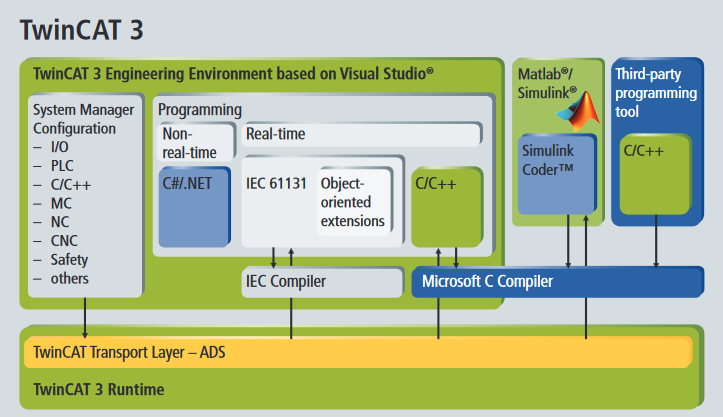
\includegraphics[width=0.90\textwidth]{Pictures/TwinCat3_Beckhoff.png}
\caption{TwinCAT 3 \citep{Beckhoff2016}}
\label{fig:TwinCAT}
\end{figure}


Die im vorherigen Abschnitt vorgestellte Statusmaschine soll mittels einer SPS Programmierung umgesetzt werden. Zur informationtechnischen Umsetzung wurde die Automatisierungssoftware TwinCAT 3 der Fa. Beckhoff verwendet. TwinCAT ist die Abkürzung von \textit{The Windows Control and Automation Technology} und  ist in die Entwicklungssoftware von Microsofts Visual Studios integriert. Über das Visual Studios wird der Programm-Code kompiliert, debugged, ausgeführt und überwacht. Sie ermöglicht es den lokalen PC mit der SPS zu verbinden. 

TwinCAT 3 unterteilt sich hauptsächlich in zwei Unterpunkte: 

\begin{itemize}
\item	\textit{eXtended Automation Engineering} (XAE)
\item	\textit{eXtended Automation Runtime} (XAR).
\end{itemize}

Abbild \ref{fig:TwinCAT} zeigt den softwaretechnischen Aufbaus von TwinCAT 3 sowie deren Schnittstellen und Unterstrukturen.

Das \textit{eXtended Automation Engineering} (XAE) ermöglicht durch ihre Orientierung an der IEC 61131-3 \footnote{IEC 61131-3:  Europäische Norm die sich mit den Grundlagen Speicherprogrammierbarer Steuerungen bezüglich Programmiersprachen befasst,} die Verwendung von folgenden Sprachen :

\begin{itemize}
\item	Anweisungsliste (AWL)
\item	Kontaktplan (KOP)
\item 	Funktionsbaustein-Sprache (FBS)
\item	Ablaufsprache (AS)
\item	Strukturierter Text (ST).
\end{itemize}

Über die Norm-Programmiersprachen hinaus, ist es möglich echtzeitfähige, externe C++-Programme als auch nicht echtzeitfähige Programme mit VB.NET  als Programmiersprache in das Projekt einzubinden. Eine weitere Software-Schnittstelle erlaubt eine Verbindung zu  Toolboxen wie \textit{MATLAB} oder \textit{Simulink}. Des Weiteren eignet sich diese Schnittstelle zur Herstellung von einer Verbindung zu Datenbank-Softwares wie zB.\textit{ MySQL} oder \textit{MariaDB}. Die erzeugten Objekte, auch Module genannt, können unabhängig von ihrer Programmiersprache, in der sie erzeugt wurden,  Daten austauschen und sich gegenseitig aufrufen. 

\textit{eXtended Automation Engineering} beinhaltet das Daten-Analyse-Programm \textit{Scope}. Wie auch TwinCAT selber ist \textit{Scope} in Microsofts Visual Studios eingebunden. Das \textit{Scope} unterteilt sich in \textit{Scope View} und \textit{Scope Server}. \textit{Scope View} erlaubt die Echtzeitdarstellung von Messdaten.  \textit{Scope Server} ist für die eigentliche Aufnahme der Daten verantwortlich.


\textit{eXtended Automation Runtime} (XAR) ist zuständig für die Kommunikation von allen angeschlossenen Geräten, Feldbussen und Busklemmen der SPS. Das (XAR) stellt eine Durchlaufung des gesamten Programmcodes sowie das Empfangen und Senden einer Busklemme-Signals innerhalb eines Zyklus sicher. Auf einer SPS können mehrere Tasks laufen. Jedem Task wird eine Dauer und eine Priorität durch den Benutzer zugeteilt. Der Task mit der höchsten Priorität wird stets als erstes ausgeführt. Auf dem verwendeten CX-9020 können maximal 4 Task ausgeführt werden. Ein Task besteht aus einem oder mehreren Programmen, Funktionen und Funktionsbausteinen.  Die Grundlage jeglicher Kommunikation ist das \textit{Automation Device Specification} (ADS). Es stellt eine geräte- und feldbusunabhängige Schnittstelle zwischen ADS-Teilnehmern dar. 

\subsection{Namensgebung der Variablen}
\label{subsec: Namensgebung}

\subsubsection{Waagen-Kommunikation mittels RS-232}
\label{subsec:RS-232}

\subsection{Modbus RTU}
\label{subsec:Modbus RTU}

\subsection{Programme}
\label{subsec:Programme}

\subsubsection*{EnthalpieBerechnen()}

\subsubsection*{SchwerpunktEis()}

\subsubsection*{Regelung()}


Beide Sensoren hatte eine fest eingestellte Stopbit-Größe. Der Drucktransmitter hat einen Stopbit, das Expansionsventil zwei.

\subsection{Grafical User Interface - GUI}
\label{subsec:GUI}


Drei Hauptzonen sind in der Abbildung farblich dargestellt. Das ist zum einen in \textit{grün} die Kompressor-Einheit. In der \textit{orange} Zone befinden sich der Verflüssiger und der Abtau-Verdampfer. Die \textit{blaue} Zone ist der Verdampfer, er befindet sich innerhalb der KK. Alle Komponenten außerhalb der blauen Zone sind außerhalb der KK installiert. 

Im Kältekreislauf sind drei Wärmeübertrager installiert: In der \textit{organgenen} Zone sind zwei Wärmeübertrager dargestellt:

\subsection{Anlagenschutz}
\label{subsec: Anlagenschutz}